\chapter{Konzepte}
Dieses Kapitel dokumentiert das Softwaredesign der siot.net Gateway Library und des siot.net Sensorcenters.
\section{Konzept - siot.net Gateway Library}
\subsection{Packagediagramm}
Das auf Abbildung 9.1 visualisierte Paketdiagramm, zeigt die Einteilung der Klassen und deren Abhängigkeiten.
\begin{figure}[H]
  \centering
  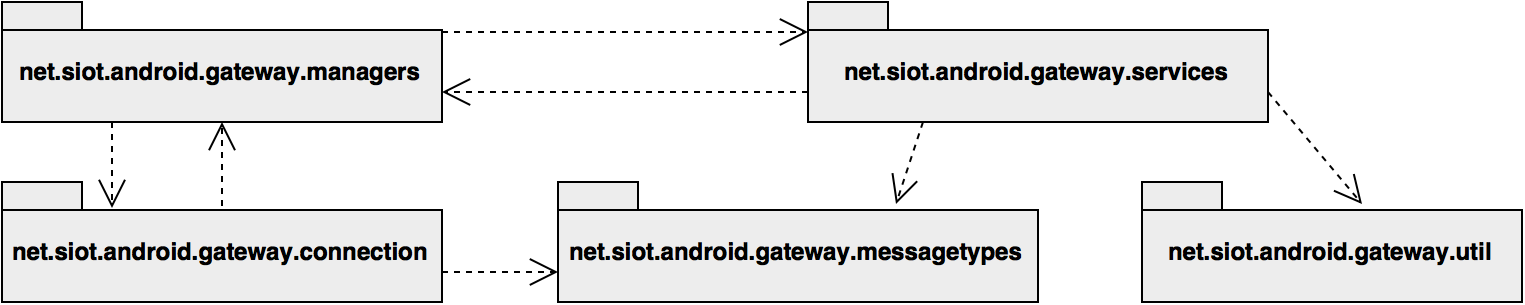
\includegraphics[scale=0.3]{98_Bilder/09_Konzept/PackagediagrammSiotNetGatewayLibrary}
  \caption[siot.net Gateway Library Packagediagramm]{Java-Package Aufteilung der siot.net Gateway Library}
\end{figure}
Die Auflistung der einzelnen Packages mit den enthaltenen Klassen (Verwendung von Entwurfsmuster sind in Klammern).
\begin{table}[H]
\centering
\begin{tabular}{p{8cm} p{8cm}}
\textbf{net.siot.android.gateway.managers}\newline
- SiotNetGatewayManager (Abstrakte Fabrikklasse)\newline
- SiotNetGatewayManagerMobile (Fabrikklasse)\newline
- SiotNetGatewayManagerWear (Fabrikklasse)\newline
- ReceivedMessageManager(Beobachtbare-Klasse)\newline
&
\textbf{net.siot.android.gateway.services}\newline
- SensorService (Abstrakte Fabrikklasse)\newline
- SensorServiceMobile (Fabrikklasse)\newline
- SensorServiceWear (Fabrikklasse)\newline
- LocationService\newline
\\
\textbf{net.siot.android.gateway.connection}\newline
- \gls{MQTT}Client (Singleton Klasse)\newline
- RestClient\newline
&
\textbf{net.siot.android.gateway.util}\newline
- GUIDUtil\newline
- TopicUtil\newline
- SensorTypeKeys\newline
\\
\textbf{net.siot.android.gateway.messagetypes}\newline
- SensorActorManifest\newline
- SensorConfig\newline
- ActorConfig\newline
- SiotUrl\newline
- Urls\newline
- WearableData & \\
\end{tabular}
\caption{siot.net Gateway Library: Auflistung der Packageinhalte}
\end{table}

\newpage
\subsection{Domänendiagramm}
Auf der folgenden Abbildung 9.2, ist das gesamte konzeptionelle Domänendiagramm der siot.net Gateway Library aufgezeichnet.
\begin{figure}[H]
  \centering
  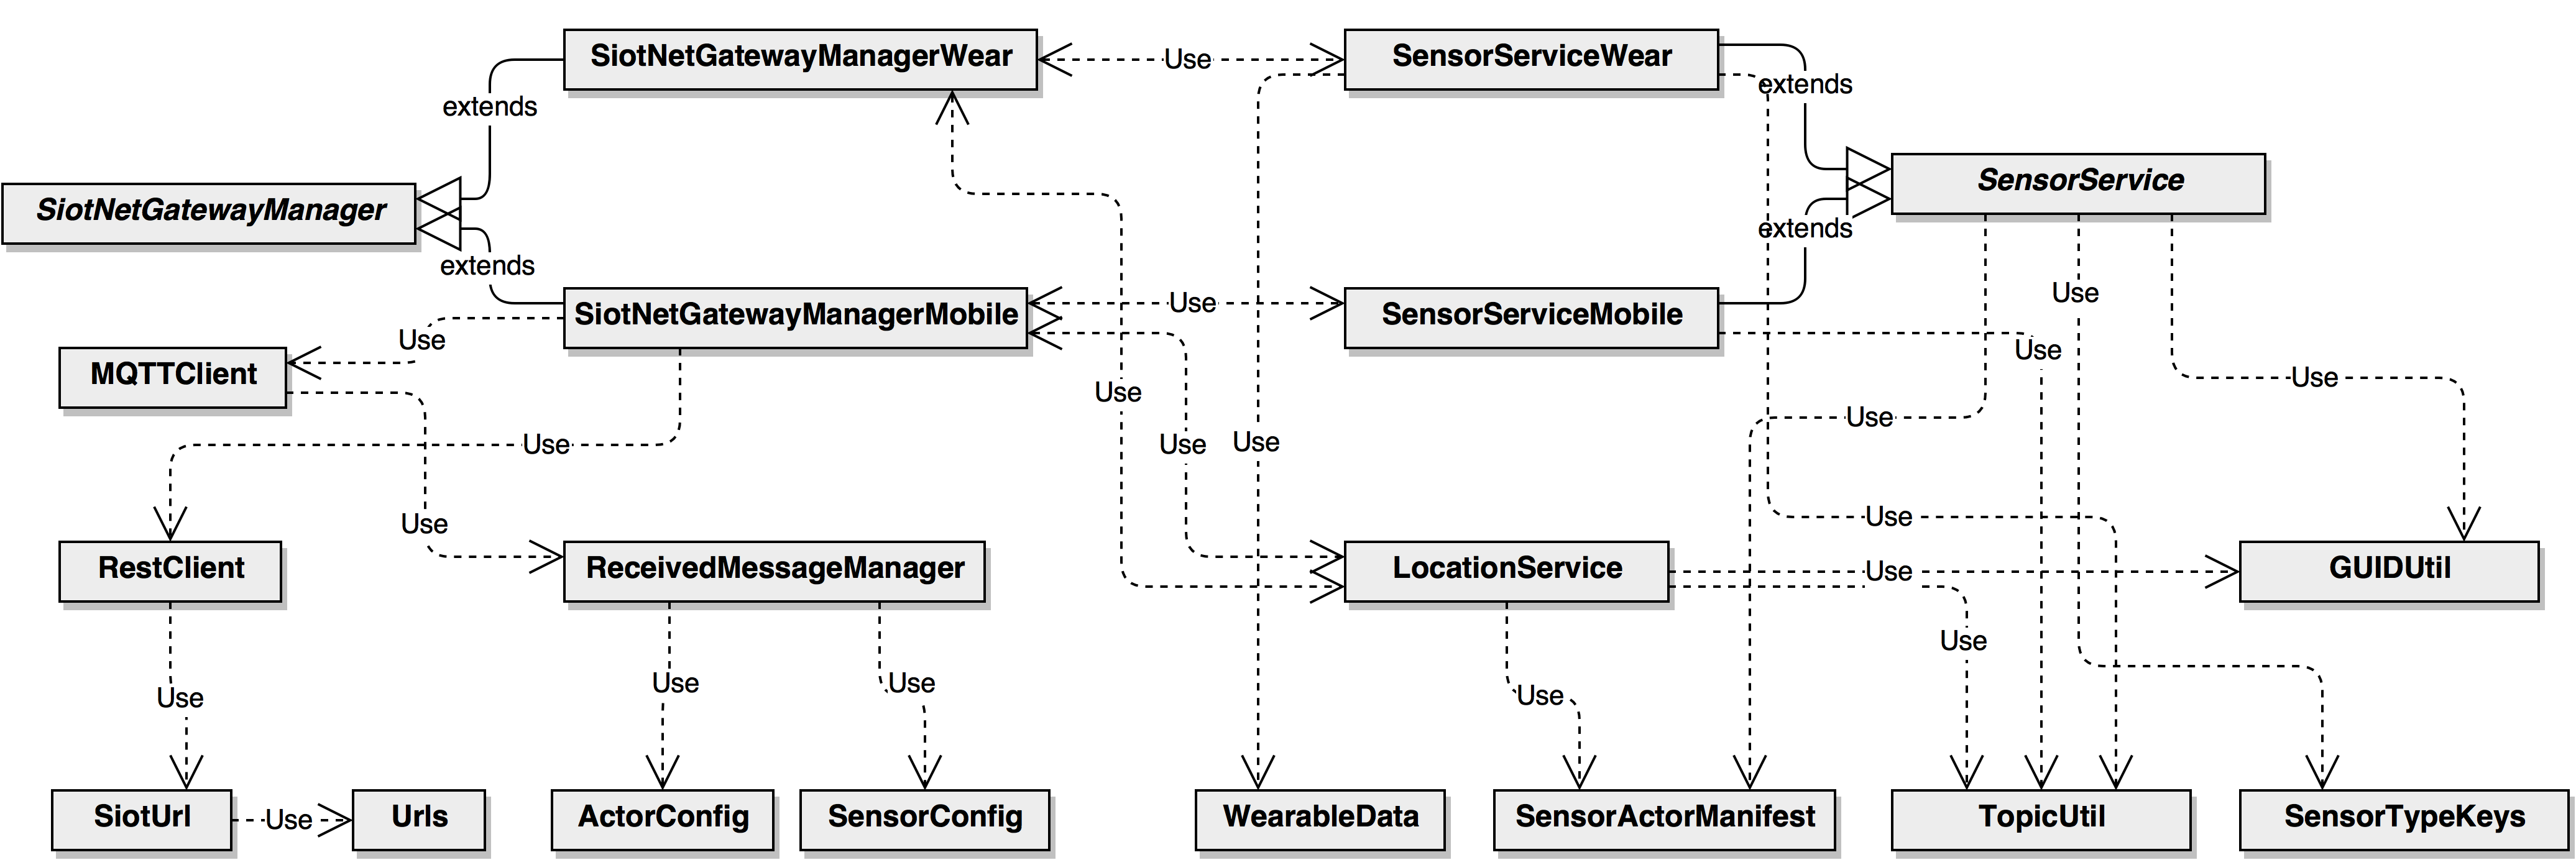
\includegraphics[scale=0.12]{98_Bilder/09_Konzept/DomaindiagrammSiotNetGatewayLibrary}
  \caption[siot.net Gateway Library Domänendiagramm]{Die Gesamtübersicht aller Klassen der siot.net Gateway Library}
\end{figure}
Apps, welche dieses Paket integrieren, instanziieren in erster Linie die Managerklassen. Die \textit{SiotNetGatewayManagers} sind in Anlehnung des Designpatterns der Fabrikmethode (vgl. \cite{gof:design_patterns} Chapter 3. Creational Patterns) konzipiert. Falls noch weitere Android Gerätearten hinzukommen, kann eine dazu passende Fabrik dazu programmiert werden (z.B. \textit{SiotNetGatewayManagerCar)}. Die \textit{ReceivedMessageManager} Klasse ist für den Gebrauch in einem Beobachter-Entwurfsmuster (vgl. \cite{gof:design_patterns} Chapter 5. Behavioral Patterns) vorbereitet. Sie ist Observable und sollte von einem Observer Objekt instanziiert werden. Von diesem Objekt darf nur eine Instanz erstellt werden. Deswegen kommt hier das Singleton-Entwurfsmuster (vgl. \cite{gof:design_patterns} Chapter 3. Creational Patterns) zur Anwendung. \\
Die Serviceklassen beinhalten die Verwaltung und die Kommunikation von den Sensoren und den Ortungsdaten. Die Sensorservices sind ebenfalls mit der Fabrikmethode konzipiert.\\
Das Connection-Paket ist für die Verbindungsobjekte zuständig. Der \textit{\gls{MQTT}Client} wird gleichwohl, wie der \textit{ReceiverMessageManager}, mit einer Singleton-Klasse angesteuert. \textit{RestClient} implementiert die statische Methode zum konsultieren des \gls{URL}-Services.\\
In Utils sind Helferklassen enthalten und in messagetypes werden die Datentypen der Kommunikation definiert.
\newpage
\subsection{Sequenzdiagramme}
Die grundlegenden Abläufe sind mit Sequenzdiagrammen spezifiziert.
\subsubsection{App starten}
Die Vorgänge, welche beim starten einer Smartphone- und Smartwatch-App durchlaufen werden, sind in der Abbildung 9.3 und 9.5 illustriert.
\begin{figure}[H]
  \centering
  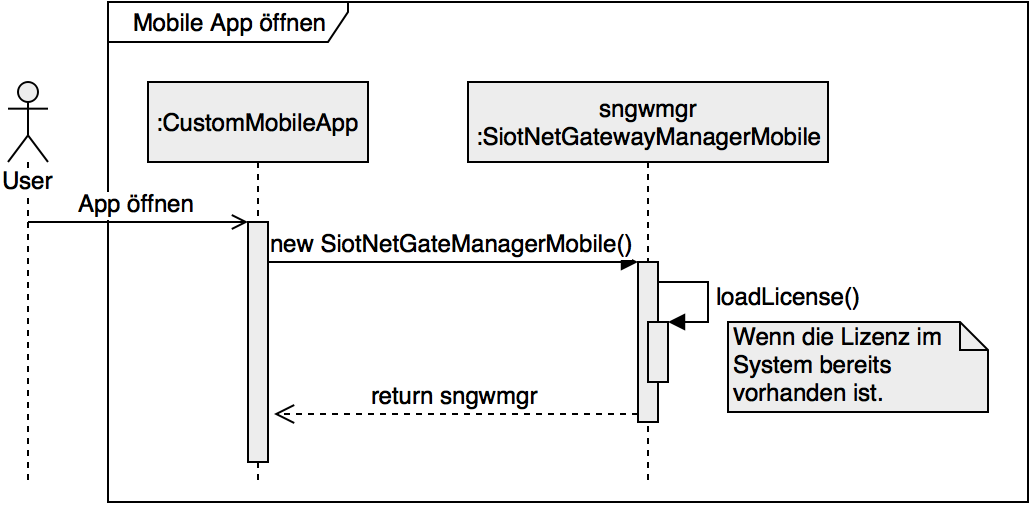
\includegraphics[scale=0.28]{98_Bilder/09_Konzept/01_SequenzdiagrammOpenAppSiotNetGatewayLibrary}
  \caption[siot.net Gateway Library Sequenzdiagramm App starten 1]{Sequenzdiagramm: Starten von Smartphone App}
\end{figure}
Das normale Starten einer Smartphone Applikation, welche die siot.net Gateway Library integriert, wird auf der Abbildung 9.3 geschildert.
\begin{figure}[H]
  \centering
  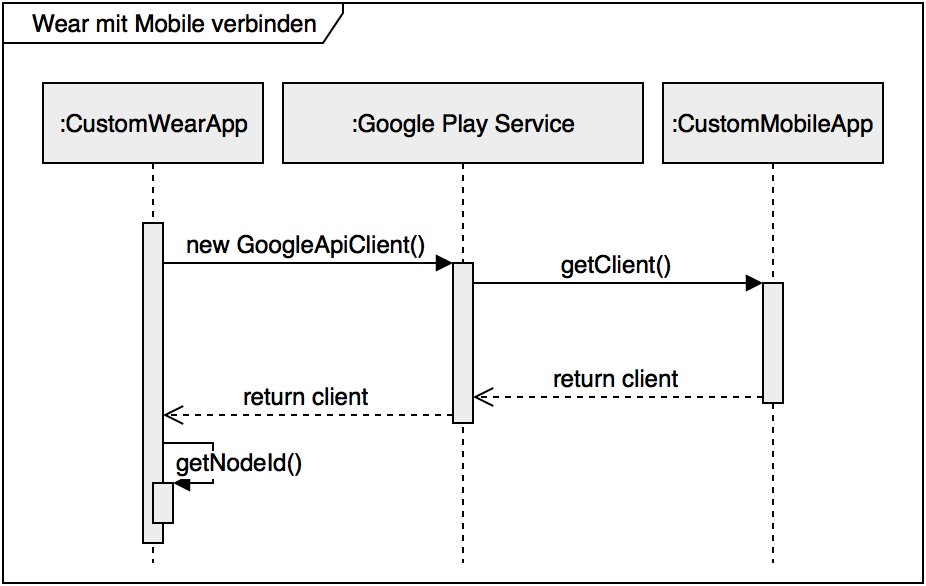
\includegraphics[scale=0.28]{98_Bilder/09_Konzept/02_SequenzdiagrammOpenAppSiotNetGatewayLibrary}
  \caption[siot.net Gateway Library Sequenzdiagramm App starten 2]{Sequenzdiagramm: Verbindungsaufbau von Smartwatch zu Smartphone}
\end{figure}
Wenn die dazugehörige Smartwatch Anwendung aufgerufen wird, welche im vorgehenden Diagramm erwähnt wurde, verbindet es sich zuerst via Google Play Service zum gekoppelten Android Smartphone. Dazu die erklärende Abbildung 9.4. Das danach folgende Sequenzdiagramm auf Abbildung 9.5 hat eine Abhängigkeit darauf.
\begin{figure}[H]
  \centering
  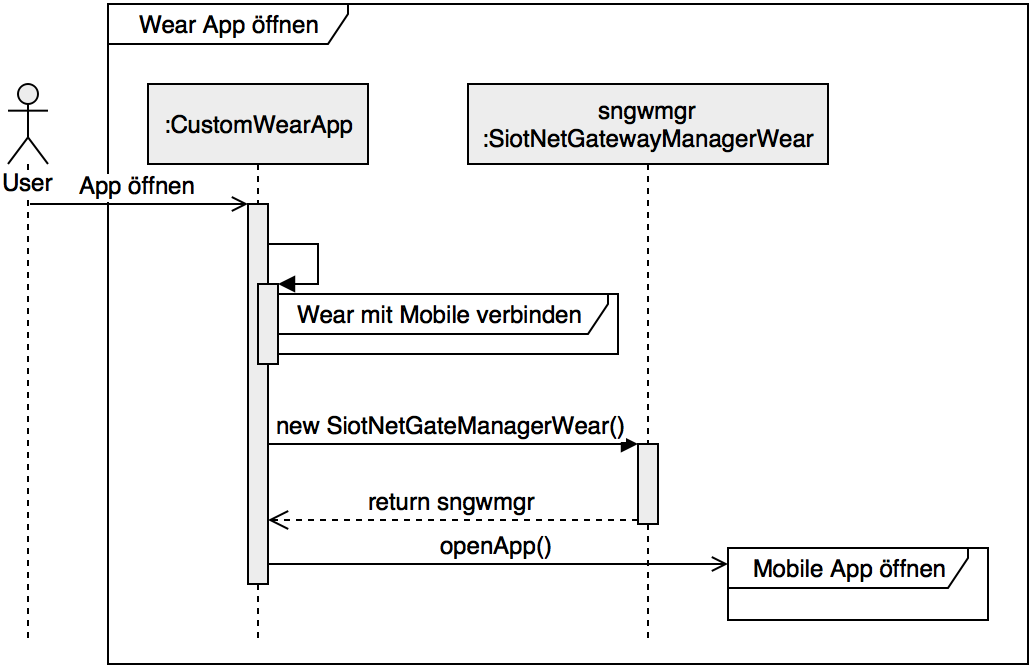
\includegraphics[scale=0.28]{98_Bilder/09_Konzept/03_SequenzdiagrammOpenAppSiotNetGatewayLibrary}
  \caption[siot.net Gateway Library Sequenzdiagramm App starten 3]{Sequenzdiagramm: Starten von Smartwatch App}
\end{figure}
Der Minicomputer am Handgelenk kann die siot.net Schnittstelle nur dann zur Verfügung stellen, wenn die Verbindung zum Smartphone aktiv ist. Zum erzeugen des Managerobjektes muss der vorher erhaltene GoogleApiClient mitgegeben werden.
\subsubsection{Login zu siot.net}
Die Kommunikationsabfolgen für das Login zum siot.net sind auf Abbildung 9.6 und 9.7 visualisiert.
\begin{figure}[H]
  \centering
  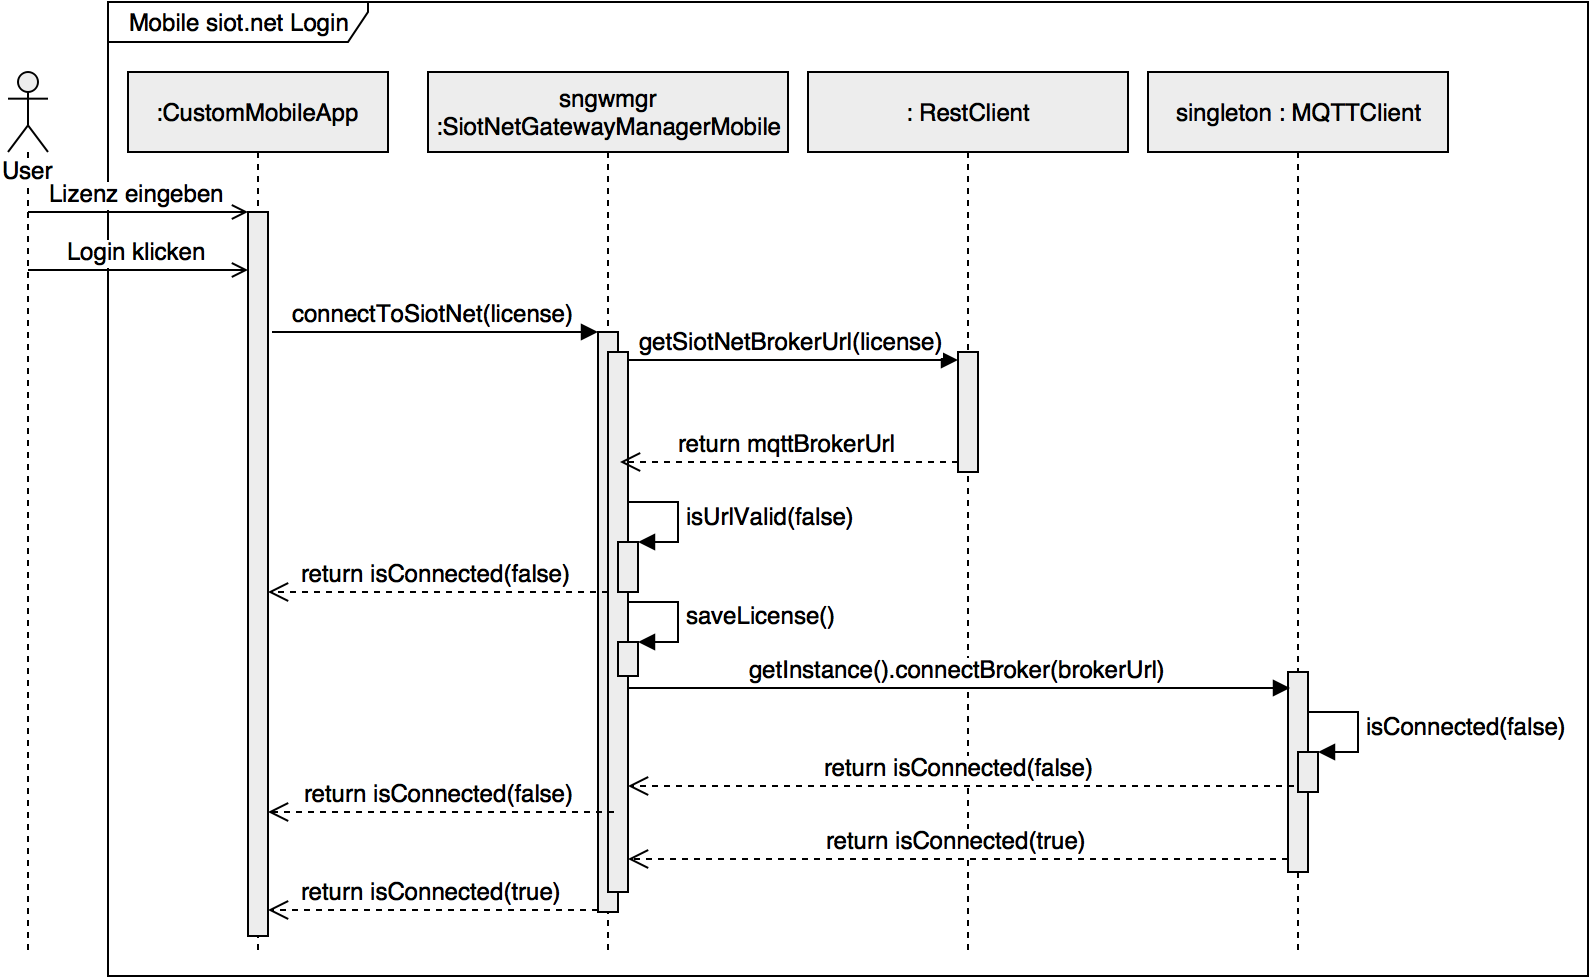
\includegraphics[scale=0.28]{98_Bilder/09_Konzept/01_SequenzdiagrammLoginSiotNetGatewayLibrary}
  \caption[siot.net Gateway Library Sequenzdiagramm Login 1]{Sequenzdiagramm: Einloggen von einer Smartphone App}
\end{figure}
Abbildung 9.6 erläutert das Loginverfahren über ein Android Mobile Gerät. Für das Login benötigt es immer einen gültigen siot.net Lizenzcode. Nach einer erfolgreichen Autorisierung beim siot.net \gls{URL}-Service, wird der Schlüssel im System in einer Konfigurationsdatei abgelegt. Dieser wird bei jedem Start geladen (siehe Abbildung 9.3). Aus dieser positiven Bestätigung kann die Adresse des \gls{MQTT} Brokers gelesen werden. Der weitere Verlauf ist auf der Abbildung 9.6 ersichtlich.
\begin{figure}[H]
  \centering
  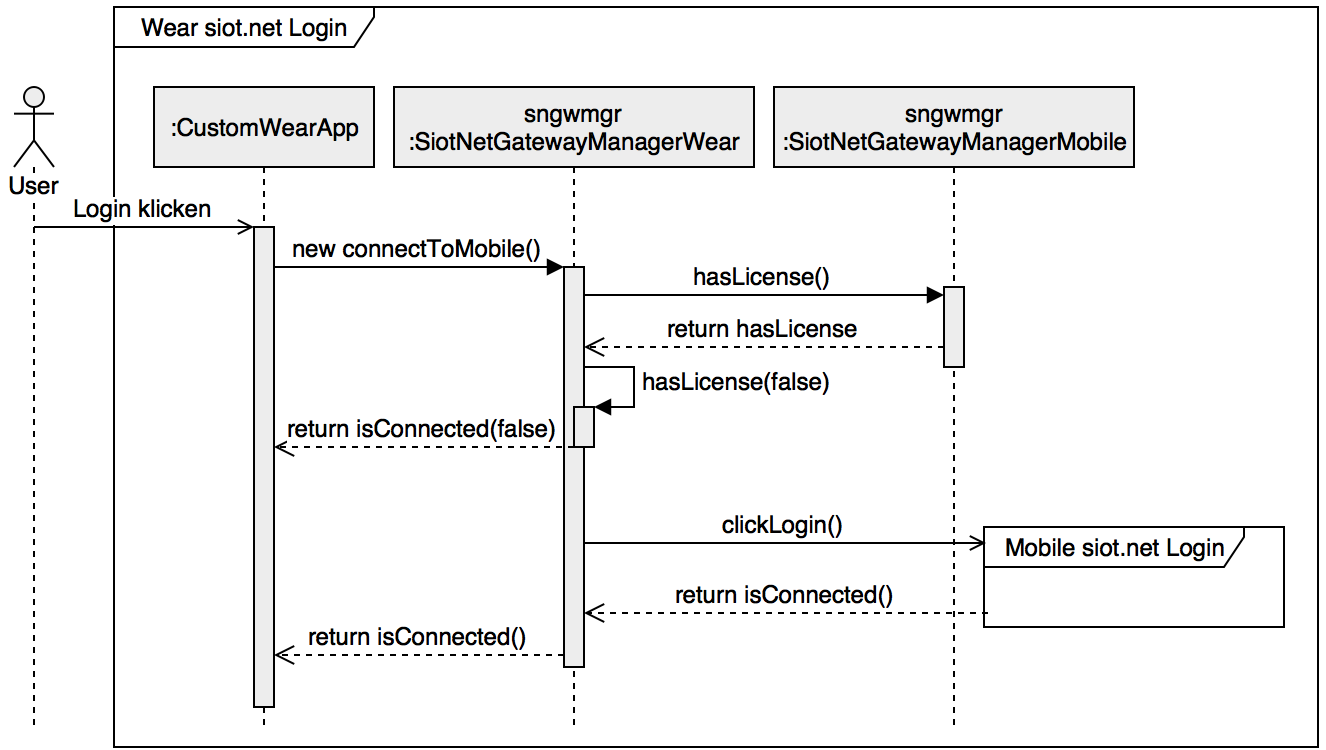
\includegraphics[scale=0.28]{98_Bilder/09_Konzept/02_SequenzdiagrammLoginSiotNetGatewayLibrary}
  \caption[siot.net Gateway Library Sequenzdiagramm Login 2]{Sequenzdiagramm: Einlogen von einer Smartwatch}
\end{figure}
Die Autorisierung via Smartwatch geschieht nur indirekt. Dieser verlangt, dass bereits ein valider Lizenzcode auf dem Smartphone existiert. Dies ist notwendig, da die Android Wear Geräte keine virtuelle Tastatur besitzen. Eine Eingabe wär nur per Sprachbefehl möglich, was die siot.net Gateway Library nicht unterstützt. Ist dieser vorhanden, fordert die Datenuhr das Smartphone dazu auf sich mit dem siot.net \gls{MQTT} Broker zu verbinden. Die Abbildung 9.7 stellt das genaue Sequenzdiagramm zu diesem Vorgang dar.
\section{Konzept - siot.net Sensorcenter}
\subsection{Domänendiagramm}
Die Abbildung 9.8, ist das Domänendiagramm vom siot.net Sensorcenter.
\begin{figure}[H]
  \centering
  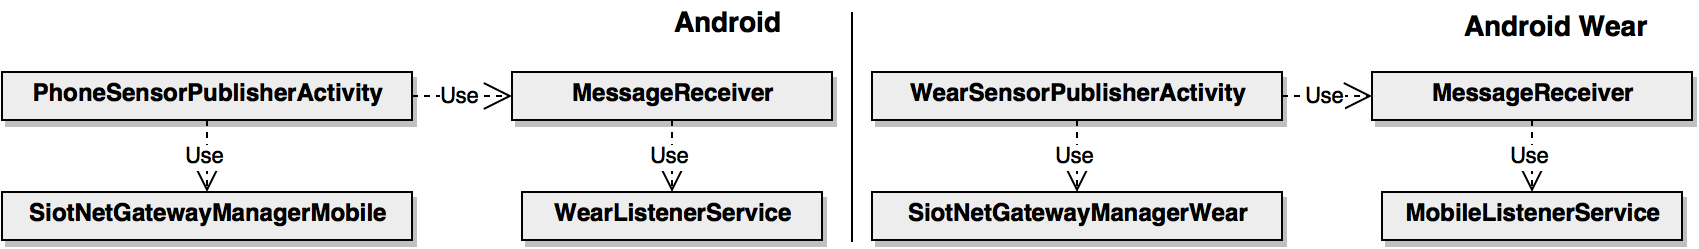
\includegraphics[scale=0.25]{98_Bilder/09_Konzept/DomaindiagrammSiotNetSensorcenter}
  \caption[siot.net Sensorcenter Domänendiagramm]{Die Klassenübersicht vom siot.net Sensorcenter im Domänendiagramm}
\end{figure}
Die Klassenstruktur der Endanwender-App kann sehr schlank gehalten werden, da die meisten Aufgaben die siot.net Gateway Library bereits erledigt. Es ist notwendig, dass zwei fast identische Applikationsstrukturen in einem Projekt bestehen. Die Wearable App differenziert sich erheblich zur Smartphone App. Des weiteren ist von Android vorgegeben, dass für die Smartphone Activity und die Watch Activity ein separates Package erstellt wird (vgl. \cite{deva:mpas}). Die Kernelemente jeweiliger Applikationen sind die Activityklassen. Diese sind zuständig für die grafische Benutzeroberfläche und instanziieren die siot.net Gateway Libraray. Das nötige Managerobjekt wird mit Hilfe der passenden Manager-Fabrik erzeugt. Der \textit{ListenerService} und der \textit{MessageReceiver} sind zuständig für die Kommunikation zwischen Smartphone und Smartwatch.
\subsection{Sequenzdiagramm}
Die folgenden Abbildungen 9.9 und 9.10 legen fest, wie die Sensorsteuerung, in Kombination mit der Gateway Bibliothek, von statten geht.
\begin{figure}[H]
  \centering
  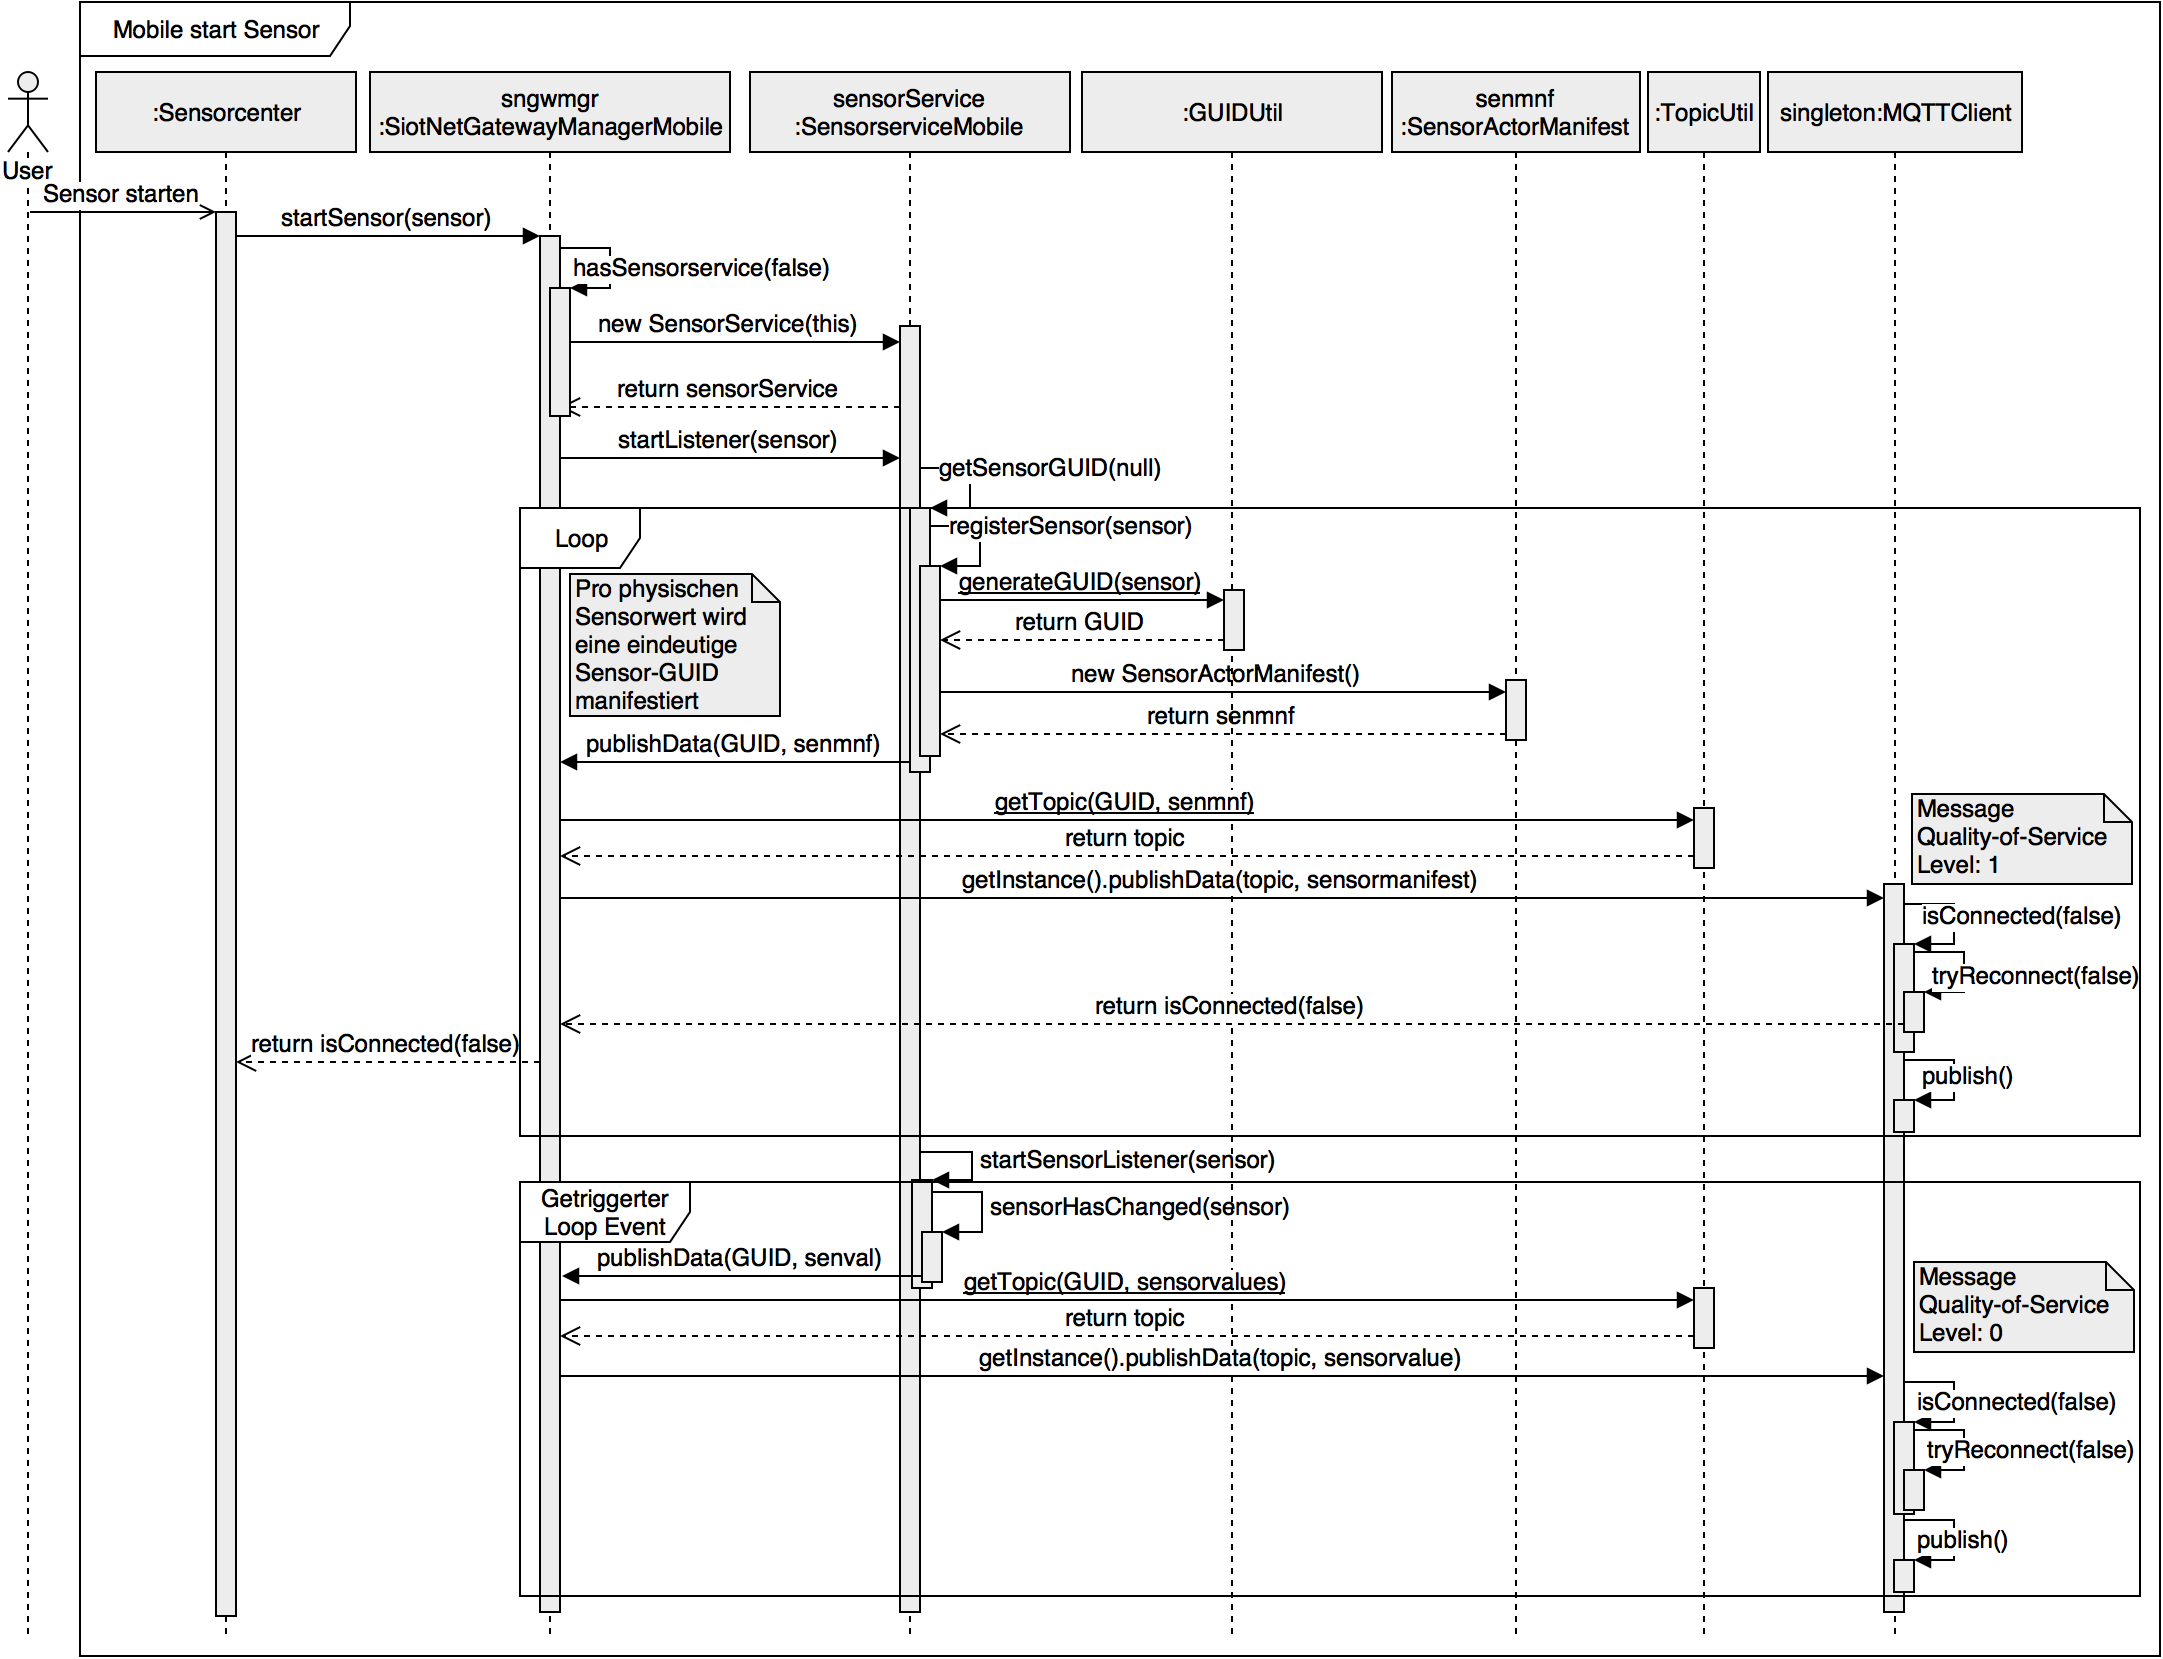
\includegraphics[scale=0.22]{98_Bilder/09_Konzept/01_SequenzdiagrammSensorstartSiotSensorcenter}
  \caption[siot.net Sensorcenter Sequenzdiagramm Sensor starten 1]{Der Ablauf beim starten eines Sensors im Sensorcenter}
\end{figure}
Die erste Spezialität in Abbildung 9.9 ist beim \textbf{Loop} Rahmen. Dieser Turnus kommt dann zum Zug, wenn der Sensor zum ersten Mal gestartet wird. Ein Sensor muss sich unter Umständen mehrfach manifestieren, aufgrund mehreren physischen Werten. Beispielsweise hat ein Beschleunigungsmesser in einem dreidimensionalen System die Werte der X-Achse, Y-Achse und Z-Achse, das heisst pro Achse wird ein Manifest des Sensors erzeugt.\\
Nach der erfolgreichen Anmeldung des Sensors, wird der, vom Android System bereitgestellten Zuhörer des Sensors, aktiviert. Dieser gibt bei jeder Veränderung des Sensors einen Messwert zurück, dass dann eine \gls{MQTT} Nachricht an den siot.net Broker auslöst. Solange der Messwertegeber nicht ausgeschaltet ist, wird nach jeder Auslösung des Sensorlisteners die Sequenz im Rahmen \textbf{Getriggerter Loop Event} durchlaufen.
\begin{figure}[H]
  \centering
  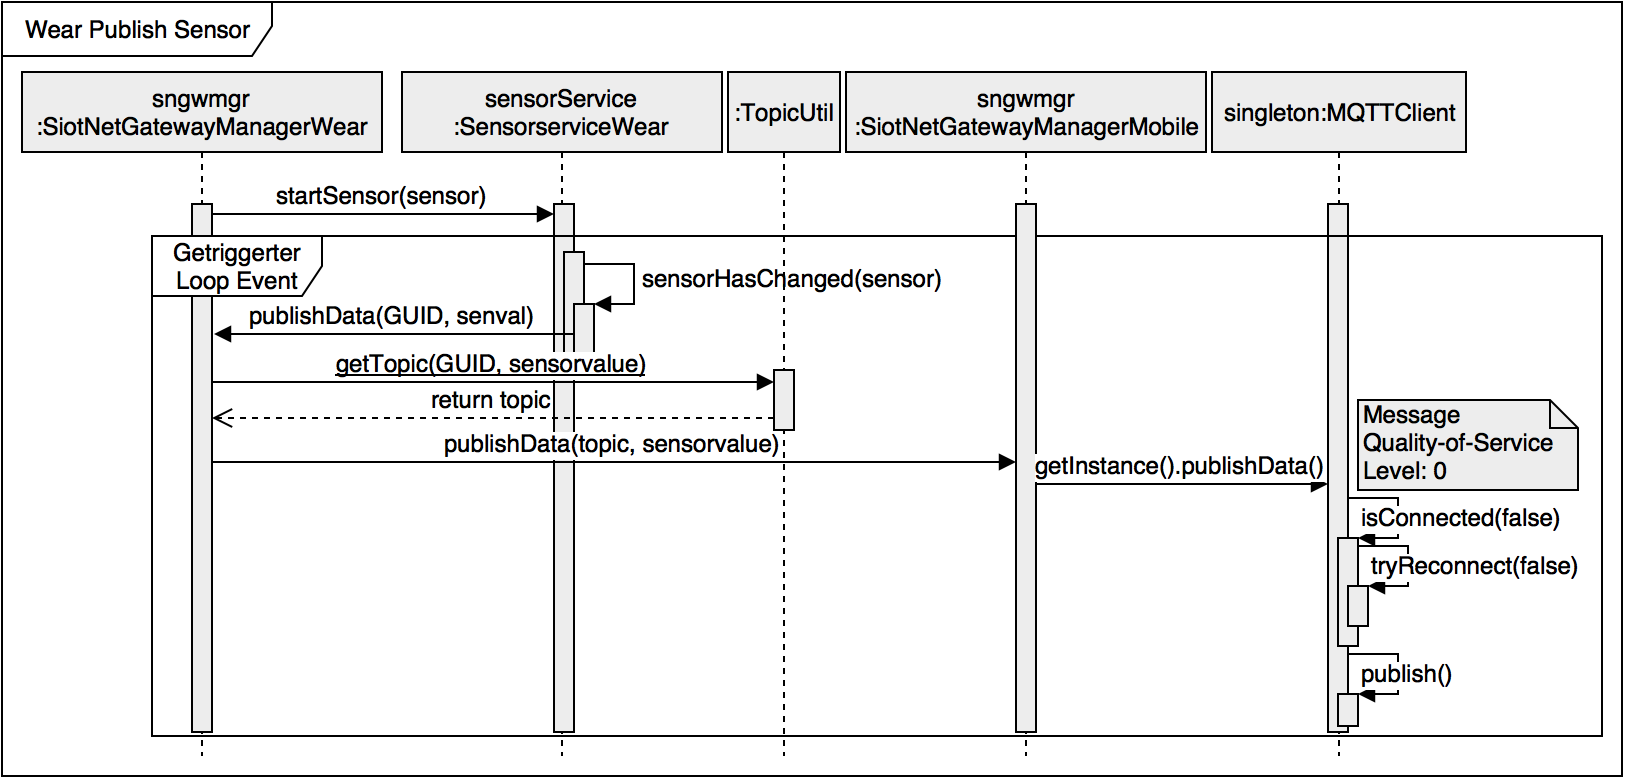
\includegraphics[scale=0.23]{98_Bilder/09_Konzept/02_SequenzdiagrammSensorstartSiotSensorcenter}
  \caption[siot.net Sensorcenter Sequenzdiagramm Sensor starten 2]{Kommunikationsverhalten beim senden von Daten bei Smartwatch}
\end{figure}
Das Auslösen von Nachrichten bei der Smartwatch benötigt noch einen weiteren Schritt. Durch die Beschränkung, dass keine Werte direkt von der Uhr ins Internet durchgestellt werden können, müssen die Datenpaket zuerst dem Smartphone zugestellt werden. Um die Informationen durchzuschleusen, wird dieses als Datenbrücke verwendet (wie auf Abbildung 7.5 und 7.6 geschildert).

\section{Konzept - Kommunikation Smartphone-zu-Smartwatch}
Für die Kommunikation von Smartphone zu Smartwatch und umgekehrt wurde ein Kommunikationskonzept zugewiesen. Die Kommunikation soll ausschliesslich über die asynchrone Schnittstelle der Android Message\gls{API} verlaufen.

\subsection{Request-Response}
Anweisungen und Informationen, welche zwischen den zwei Geräten ausgetauscht werden, müssen im Request-Response Verfahren ablaufen. Dies ist notwendig, weil Aktionen des einen Gerätes, Einfluss auf das Andere haben kann. Kommunikation und Funktionalität auf der Smartwatch sind stark gebunden mit dem Status des Smartphones. Darum müssen die Messages gegenseitig quittiert werden. Die Message-Struktur und -Inhalt ist durch den individuellen Entwickler selber zu bestimmen. Es ist eine synchrone Kommunikation über eine asynchrone Schnittstelle. Dies wird auch öfters als sync-over-async betitelt.
Um eine rein synchrone Schnittstelle zu erhalten kann auch die Client\gls{API} aus den Google Play Services genutzt werden. Je nach Umfang der synchronen Daten ist dies sinnvoll. Der Vorteil des sync-over-async ist, dass die Daten nicht auf dem System persistent vorhanden sein müssen. Die aus den Nachrichten erfolgenden Aktionen sind immer ereignisorientiert.

\subsection{Fire-and-Forget}
Bei den Sensormesswerten der Smartwatch ist es anders geregelt. Diese werden im Fire-and-Forget-Verfahren verschickt. Das bedeutet, die Daten werden ausgesendet aber werden nicht verfolgt oder kontrolliert, ob diese korrekt übermittelt wurden. Dies wird angewendet, weil es systemunkritische Informationen sind. Dadurch kann Energie und Bandbreite gespart werden. Ausnahme: Wenn bei der \gls{MQTT} Kommunikation, der Quality-of-Service > 0 wird (1 oder 2), sollten die Messwerte von der Smartwatch im Nachrichtenaustauschmuster Request-Response übergeben werden. Sonst kann keine Verifikation durchgeführt werden ob die Nachricht angekommen ist.

%\section{Konzept - siot.net Dashboard}
